\clearpage % Rozdziały zaczynamy od nowej strony.

%\section{Summary}
\section{Summary and conclusions}

The goal of this work was to run PenPoint OS on a modern computer with
reasonable performance, and be able to use it with the help of a mouse,
a graphics tablet or a touchscreen. PenPoint was an important and influential,
albeit now mostly forgotten piece of computing history. It is important to
preserve it and at the same time maybe gain a little insight.

%The first approach consisted of trying to port modifications of the JPC
%emulator created by professor Simon Schubiger to the QEMU hypervisor. The JPC
%emulator was not performant enough to run PenPoint OS at a speed that would be
%comfortable to use. First the changes to the JPC emulator required to run
%PenPoint were discussed in detail: what they do, how they do it, and how all of
%this relates to the general architecture of the JPC. Then the operation of the
%QEMU hypervisor, the process of defining a new device in the QEMU source tree
%and making it available to QEMU, and the reasoning behind choosing QEMU were
%described in depth. This approach however was abandoned because of the
%complexity and because an easier way became available.

The first approach consisted of trying to port modifications of the JPC
emulator created by professor Simon Schubiger to the QEMU hypervisor.  The JPC
emulator was not performant enough to run PenPoint OS at a speed that would be
comfortable to use.  First, the changes to the JPC emulator required to run
PenPoint were discussed in detail: what they do, how they do it, and how all of
this relates to the general architecture of the JPC.  Then the operation of the
QEMU hypervisor, the process of defining a new device in the QEMU source tree
and making it available to QEMU, and the reasoning behind choosing QEMU were
described in depth.  This approach, however, was abandoned because it was deemed
unnecessarily complex, and outside of the scope of this work.  Instead, a more
straightforward and less error prone solution was chosen.

\begin{figure}[!h]
    \centering
    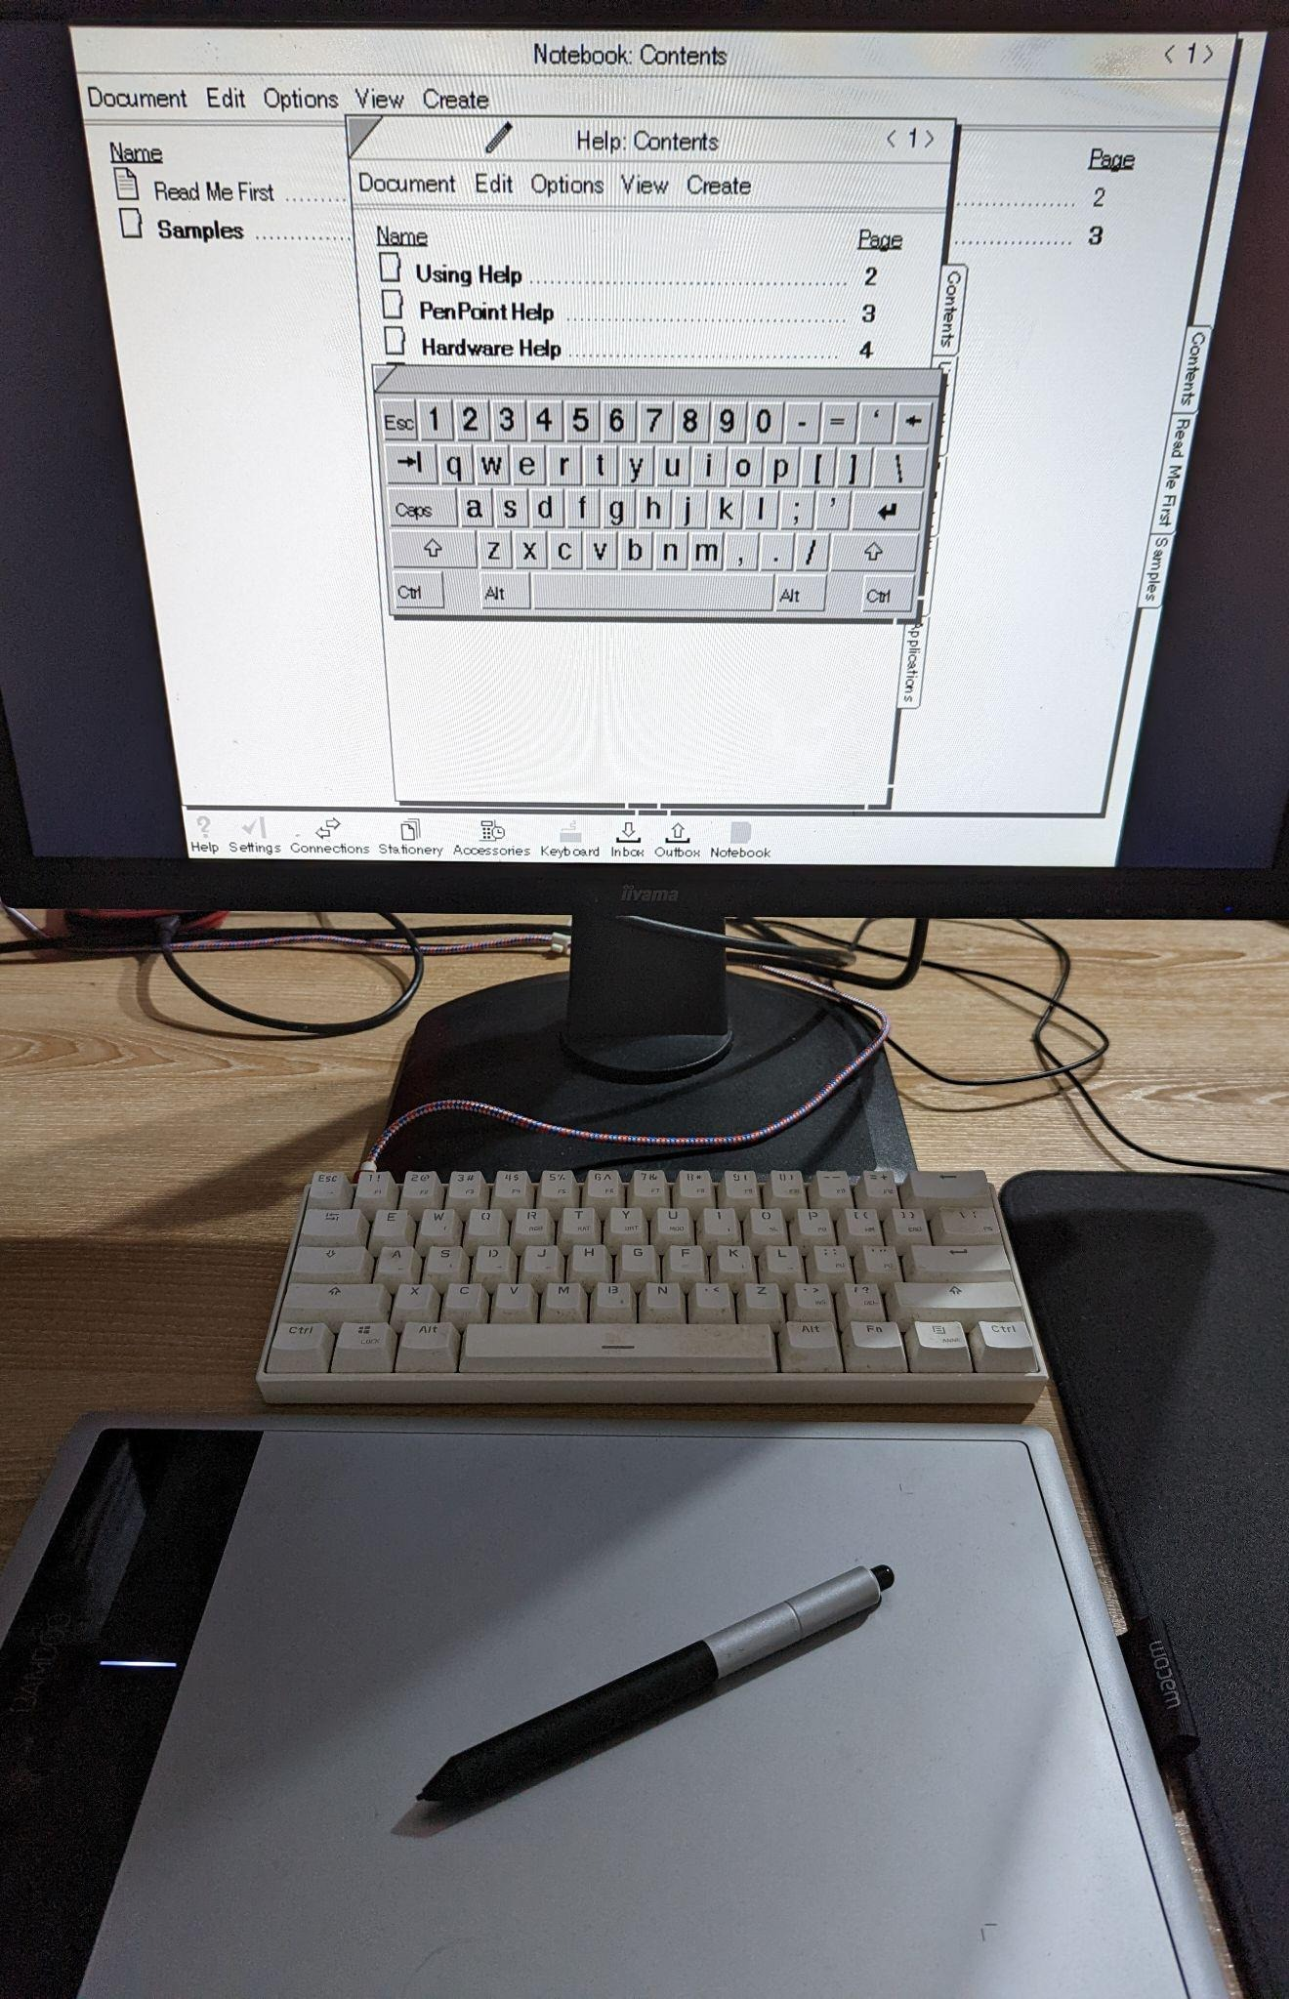
\includegraphics[width=0.9\linewidth]{penpoint-pc-tablet.png}
    \caption{PenPoint OS running on PC with a graphics tablet}
    \label{fig:penpoint-pc-tablet}
\end{figure}

In the second approach, a different distribution of PenPoint OS was used, one
that was created so that it could be installed on a PC running MS-DOS.  Here the
process of obtaining the installation files, the installation, and configuration
of the DOS environment created using FreeDOS, and of PenPoint was described.
First it was described how the SDK distribution of PenPoint differs from the
version created for the NCR 3125.  Then it was shown how the floppy disk files
ought to be prepared to be used with a virtual machine, and the process of
installation was explained.  Finally it was demonstrated how to configure the
FreeDOS environment to run PenPoint OS and how to configure PenPoint OS itself
to work with a mouse.  The difference between a relative and absolute pointing
device was discussed as well.  Finally the process of handling mouse and tablet
input in QEMU was described, as well as the implementation of adding the
absolute pointing mode functionality, and how the conversion from absolute
values to relative values is performed in the PS/2 mouse QEMU device.

%, how it works in both QEMU and VirtualBox, and what
%was tried and what should be done in QEMU to support an absolute pointing device
%like a graphics tablet.

% conclusions
The original goal of running PenPoint OS on modern hardware was met
\ref{fig:penpoint-pc-tablet} by using the SDK distribution of PenPoint and
installing it on FreeDOS in a modified version of QEMU.

\begin{itemize}
    \item
        It is possible to run PenPoint on any computer that can run QEMU
    \item
        The performance of this solution is excellent
    \item
        It is possible to use a graphics tablet or a touch screen as a pointing
        device
\end{itemize}

%Potential improvements include modifying source code of QEMU so that absolute
%pointing methods work with it correctly, and porting the changes to JPC
%emulator created by professor Schubiger to either VirtualBox or QEMU to run the
%PenPoint OS version for NCR System 3125 - the flagship PenPoint device - with
%all of its bells and whistles.

Potential improvements include creating a QEMU device that would represent
a graphical tablet from the era.  This would not change the functionality
of the solution but it would be more `authentic' and complete.  Modifying QEMU
to run the NCR 3125 version of PenPoint, instead of the developer version, could
also prove beneficial, as it was the flagship PenPoint device that offered THE
experience that creators of PenPoint intended.  It could also be useful to use
outside of PenPoint of other software that was created for System 3125.


